%%% Local Variables:
%%% mode: latex
%%% TeX-master: "../cheat-sheet"
%%% End:

% 14. You can explain in your own words and in text and with your own commented examples, how message passing can be used to coordinate processes.

Message passing in its simplest form is given by the two constructs \texttt{send} and \texttt{receive}, which could have signatures similar to

\begin{lstlisting}
void send(int process_id, string msg)
string receive(int process_id)
\end{lstlisting}

The semantics of the operations differ, for instance calling \texttt{receive} before \texttt{send} could either block until a message is available or return an error. If \texttt{recieve} waits for a call to \texttt{send} and vice versa it is called a \textbf{rendezvous} implementation.

An \textbf{important} issue to consider is how to establish connection between sender and receiver. It could be via a lookup by process name, hardcoded, manually set by user, via network names, stdin/stdout etc.

See figure~\ref{fig:msg-passing}: Code example from Tanenbaum p. 143
\begin{figure}[h]
  \centering
  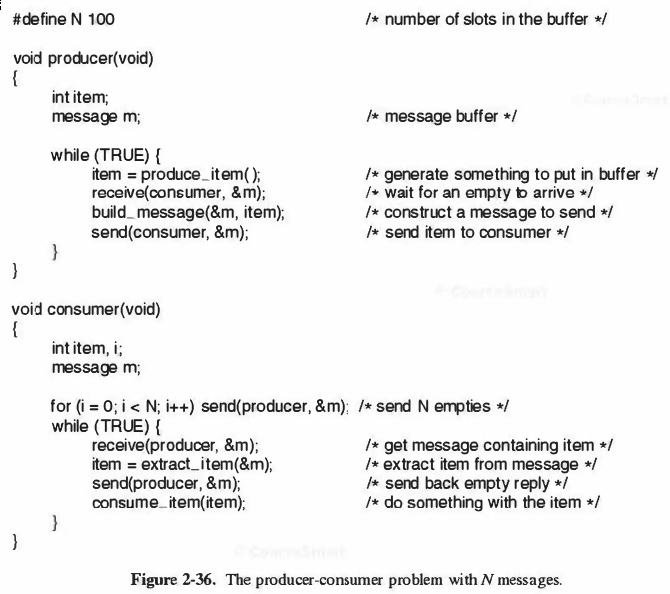
\includegraphics[width=0.8\textwidth]{images/message_passing}
  \caption{Producer/consumer via message example. From Tanenbaum.}
  \label{fig:msg-passing}
\end{figure}
